%!TEX root = ../report.tex
\section{Spinup}

Starting from $\eta = 0$ with the trivial solution satisfying equation~\eqref{eq:pde}, we apply continuation in $\eta$ from $0$ to $1$ in steps of $\Delta s = 0.1$ and find a non-trivial solution at $Re = 16$ as shown in Figures~\ref{fig:question_a_psi} and~\ref{fig:question_a_zeta}.

\begin{figure}[h!]
    \centering
    
    \centerline{
    \begin{subfigure}[b]{0.6\textwidth}
        \includegraphics[width=\textwidth]{images/a_psi.eps}
        \caption{Streamfunction $\psi$ at $Re = 16$.}
        \label{fig:question_a_psi}
    \end{subfigure}
    ~
    \begin{subfigure}[b]{0.6\textwidth}
        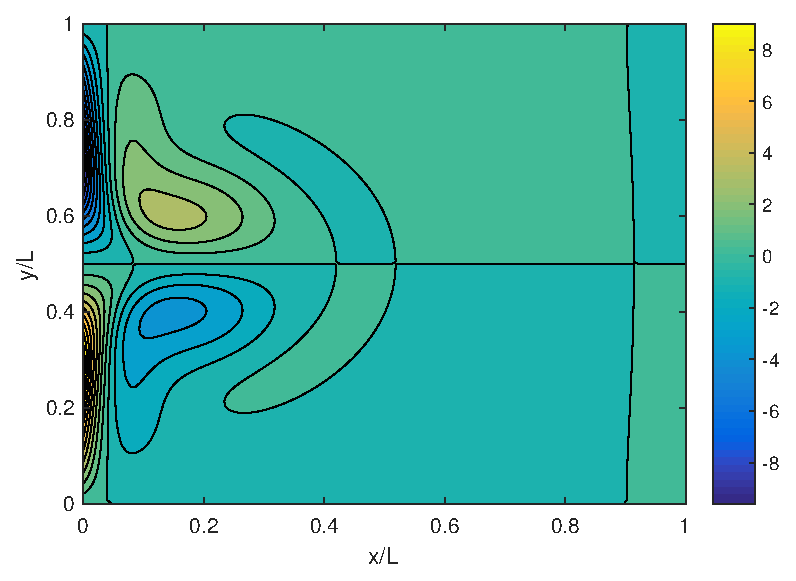
\includegraphics[width=\textwidth]{images/a_zeta.eps}
        \caption{$\zeta$ at $Re = 16$.}
        \label{fig:question_a_zeta}
    \end{subfigure}
    }
    \caption{First non-trivial solutions after spin-up.}\label{fig:question_a}
\end{figure}